% !TEX root = ./Basilisk-dvAccumulation-2019-03-28.tex


\begin{figure}[h]
	\centerline{
		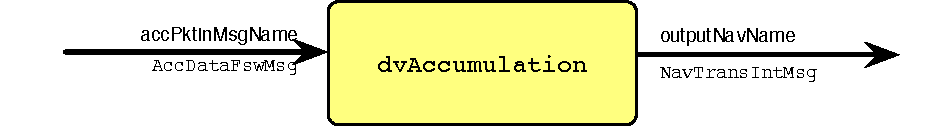
\includegraphics{Figures/moduleImg}
	}
	\caption{Illustration of the module input and output messages.}
	\label{fig:moduleImg}
\end{figure}


\section{Model Description}
\subsection{General Formulation}
In input message contains an array of accelerometer measurements $\leftexp{B}{\bm a_{i}}$ with an associated time tag $t_{i}$.  The data sets are not assumed to be ordered or sorted in chronological order.  The goal of the module is to determine the time between measurements and use a first order integration of the acceleration vector to compute the net $\Delta\bm v$ vector that has occurred.


\subsection{Reset() Functionality}
The reset function has a few critical behaviors.  
\begin{itemize}
	\item The vector containing the net $\Delta \bm v$ is zero on reset.
	\item The prior time tag $t_{n-1}$ is zero to zero on default.
	\item The input message is read and sorted it to see if the array of accelerometer data contains any time-tagged measurements already.  If yes, the prior measurement time tag $t_{n-1}$ is set to the latest data time tag $t_{i}$.  This has the effect of ensuring that when the accelerometer integration starts in the update function none of the data that existed during the reset function will be use.  In other words, old accelerometer data will not be used and only data after the reset function is considered.
	\item The initialization flag is set to false (i.e. 0).
\end{itemize}


\subsection{Update() Functionality}
The update function reads in the latest accelerometer data input message and must process all the new measurements since the last update function call.  
\begin{itemize}
	\item The accelerometer input message is read in and sorted by the time tags.
	\item If the initialization flag is not true, then the integration is occurring for the first time.  To avoid large $\Delta t$ evaluations because of an old prior time $t_{n-1}$, the input data is looped over from the end of the array (i.e. from the newest to oldest) to find the first data time tag $t_{i}$ which is newer then the prior data time tag $t_{n-1}$.  Once found we set $t_{n-1} = t_{i}$, set the initialization flag to true and break the loop.  As a result the first new data set is not included in the $\Delta\bm v$ evaluation.
	\item The next step is to loop over all data sets and see if $t_{i}>t_{n-1}$.  If yes, the associate data set has not been processed and it is integrated using $$\leftexp{B}{\Delta\bm v} += \leftexp{B}{\bm a_{i}} \Delta t$$ where $\Delta t = t_{i} - t_{n-1}$.  The prior time is set to the $t_{i}$ current data time and the loop is repeated.
	\item The final step before writing the output message is to zero all output message data and then set the {\tt timeTag} to the latest accelerometer measurement time tag, and copy over the $\Delta\bm v$ vector.
\end{itemize}